\documentclass[a4paper, 10pt]{report}
\usepackage[italian]{babel}
\usepackage[T1]{fontenc}
\usepackage[utf8]{inputenc}
\usepackage{charter}
\usepackage{amsmath}
\usepackage{amsthm}
\usepackage{amsfonts}
\usepackage{graphicx}
\usepackage{wrapfig}
\usepackage{tcolorbox}
\usepackage{fancyhdr}
\usepackage{listings}

\usepackage{geometry}
\geometry{a4paper, left=2cm,right=2cm,top=2cm,bottom=2cm}

\pagestyle{fancy}
\lhead{}
\chead{}
\rhead{\bfseries 17 ottobre 2019 }
\lhead{\bfseries Linguaggi}

\begin{document}

\section*{\underline{Espressioni}}

Un'espressione rappresenta un valore, solitamente vincolato ad un tipo. Per poter associare un valore ad un'espressione, questa deve essere valutata. I valori rappressentabili dalle espressioni sono detti \textbf{esprimibili}:
\begin{center}
$Eval = bool \cup int$ (ovvero i terminali della grammatica)
\end{center}

\noindent Le caratteristiche principali delle espressioni sono:
\begin{itemize}
\item[-] Arietà, che indica il numero di operatori ai quali si applica l'espressioni (es: arietà 2 == operatore binario);
\item[-] Tipo di notazione, che può essere infissa, suffissa o postfissa;
\item[-] Regole di associatività e precedenza (es: ordine di precedenza tra operatori dello stesso livello);
\item[-] Ordine di valutazione degli operatori (es: da sinistra verso destra);
\item[-] Generazione di side-effects;
\item[-] Possibilità di overloading delgi operatori;
\item[-] Possibilità di accettare tipi misti.
\end{itemize}

\subsection*{Notazione}

A seconda di come si rappresenta l'espressione varia il modo in cui si determina la semantica e di conseguenza la sua valutazione. La notazione infuisce anche sulle regole di associativittà e precedenza.

\paragraph*{Notazione postfissa} La notazione postfissa viene valutata usando una pila LIFO, secondo il seguente algoritmo:
\begin{enumerate}
\item Leggi il prossimo simbolo dell'espressione;
\item Se simbolo == operatore:
	\begin{itemize}
	\item[-] Applica l'operatore agli operandi  in cima alla pila e poi cancellali;
	\item[-] Memorizza il risultato in cima alla pila.
	\end{itemize}
	Se il simbolo letto è un operando inseriscilo in cima alla pila;
\item Torna a $(1)$.
\end{enumerate}

\noindent Esempio:
\begin{center}
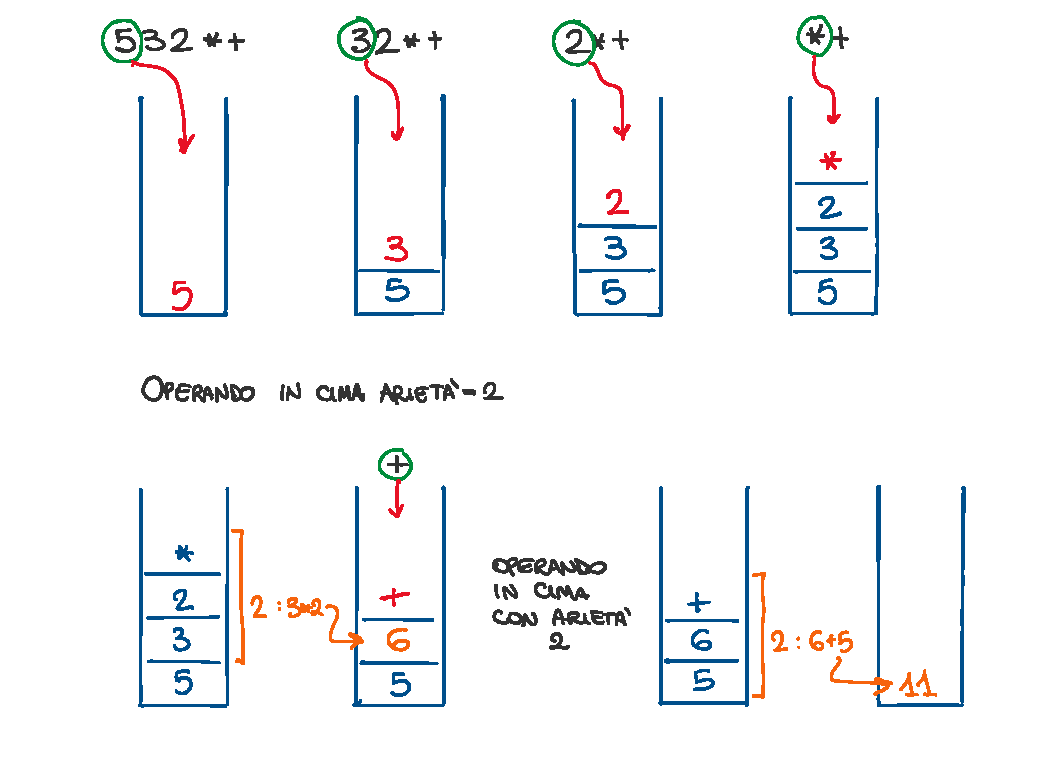
\includegraphics[scale=0.65]{esempio1.pdf}
\end{center}

\paragraph*{Notasione prefissa} La notazione prefissa non necessita di regole di associatività e parentesi. Viene valutata come segue:
\begin{enumerate}
\item Leggi il prossimo simbolo dell'espressione e mettilo in cima alla lista;
\item Se simbolo == operatore, inizializzo una variabile $C$ con l'arietà dell'operatore.
	
Se il simbolo letto è un operando inseriscilo in cima alla pila e decrementa l'operatore ($C--$);
\item Se $C \ne 0$, torna a $(1)$;

Se $C == 0$:
	\begin{itemize}
	\item[-] Applica l'operatore agli operandi in cima alla pila e poi cancellali;
	\item[-] Salva il risultato in cima alla pila;
	\item[-] $C = n - m$, con $n$ arietà del nuovo operatore in cima alla pila e $m$ numero operandi sopra l'operatore.
	\end{itemize}
\item Se la pila non è vuota, torna a $(1)$.
\end{enumerate}

\noindent Esempio:
\begin{center}
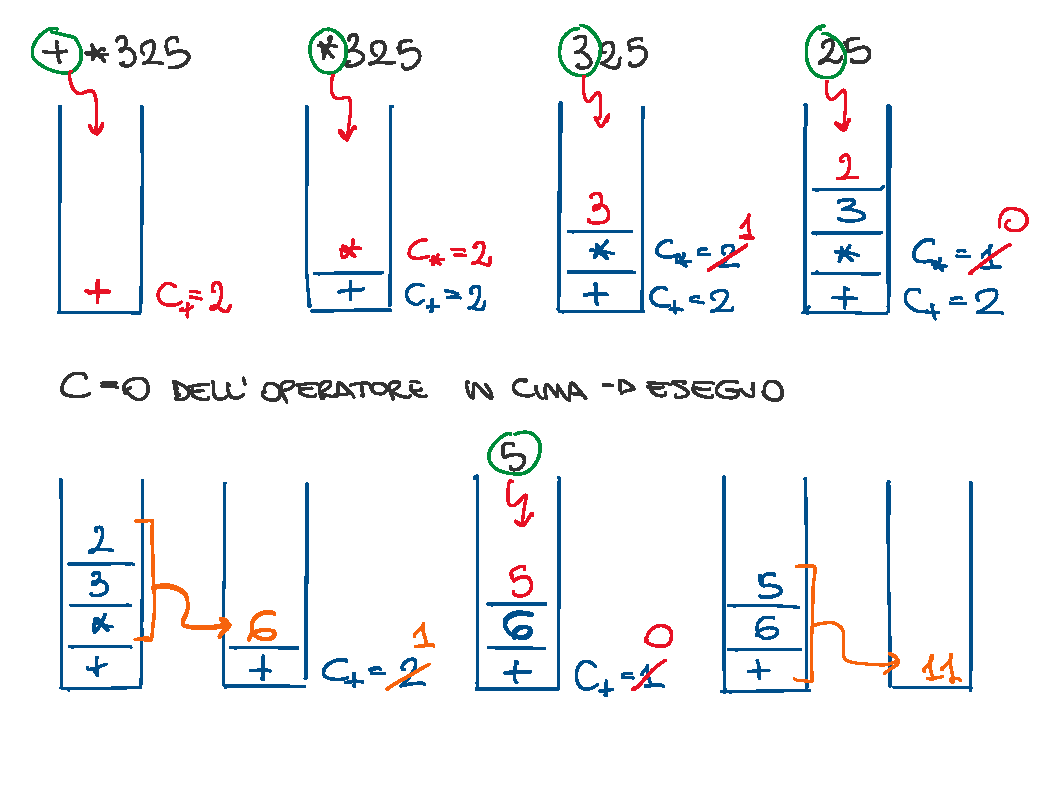
\includegraphics[scale=0.65]{esempio2.pdf}
\end{center}

\subsection*{Ordine di valutazione}
I principali problemi legati all'ordine di valutazione si hanno a causa di: operandi non definiti, effetti collaterali e aritmetica finita.

\paragraph*{Operandi non definiti} Se devo valutare la seguente espressione $a == 0 ? b : b/a$, posso avere dei problemi calcolo il risultato di $b/a$ se $a = 0$. Il problema si pone solo se ho una valutazione totatle degli operandi. 

La valutazione può essere:
\begin{itemize}
\item[-] Lazy, ovvero valuta solo gli operandi necessari. Nel caso sopra, se $a == 0$ valuta solo $b$;
\item[-] Eager, ovvero valuta tutti gli operandi a prescindere dal risultato.
\end{itemize}

\paragraph*{Generazione di effettu collaterali} Se devo valutare il seguente codice:
\begin{lstlisting}
a = 10;
b = a + fun(a);

fun(a) = a++;
\end{lstlisting}

\noindent Se valuto prima $fun(a)$ ottengo come risultato finale $b = 11 + 11$.

\noindent Se valuto prima $a$ ottengo $b = 10 + 11$.

\paragraph*{Aritmetica finita} il problema si pone quando eseguo operazioni sul massimo numero rappresentabile.


\end{document}